\documentclass{standalone}
\usepackage{tikz}
\usetikzlibrary{patterns, positioning}


\begin{document}
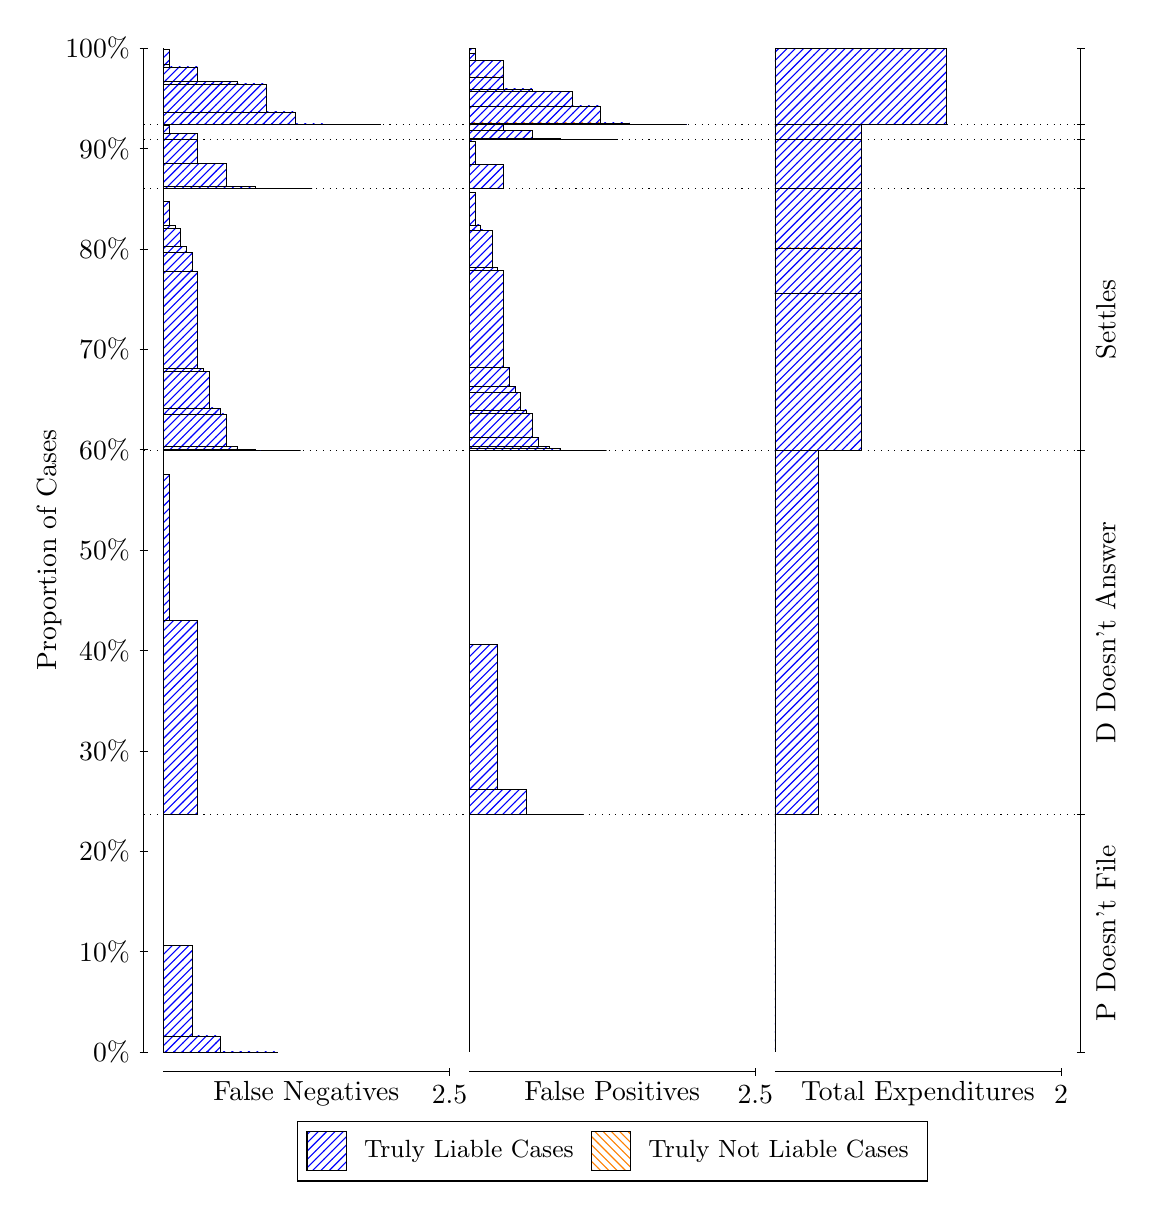
\begin{tikzpicture}
\draw[black, very thin] (1.5,1.75) -- (1.5,14.5);
\node[rotate=90, text=black, anchor=center] at (0.3, 8.125) {Proportion of Cases};
\draw[black, very thin] (1.45,1.75) -- (1.55,1.75);
\node[text=black, anchor=east] at (1.45, 1.75) {0\%};
\draw[black, very thin] (1.45,3.025) -- (1.55,3.025);
\node[text=black, anchor=east] at (1.45, 3.025) {10\%};
\draw[black, very thin] (1.45,4.3) -- (1.55,4.3);
\node[text=black, anchor=east] at (1.45, 4.3) {20\%};
\draw[black, very thin] (1.45,5.575) -- (1.55,5.575);
\node[text=black, anchor=east] at (1.45, 5.575) {30\%};
\draw[black, very thin] (1.45,6.85) -- (1.55,6.85);
\node[text=black, anchor=east] at (1.45, 6.85) {40\%};
\draw[black, very thin] (1.45,8.125) -- (1.55,8.125);
\node[text=black, anchor=east] at (1.45, 8.125) {50\%};
\draw[black, very thin] (1.45,9.4) -- (1.55,9.4);
\node[text=black, anchor=east] at (1.45, 9.4) {60\%};
\draw[black, very thin] (1.45,10.675) -- (1.55,10.675);
\node[text=black, anchor=east] at (1.45, 10.675) {70\%};
\draw[black, very thin] (1.45,11.95) -- (1.55,11.95);
\node[text=black, anchor=east] at (1.45, 11.95) {80\%};
\draw[black, very thin] (1.45,13.225) -- (1.55,13.225);
\node[text=black, anchor=east] at (1.45, 13.225) {90\%};
\draw[black, very thin] (1.45,14.5) -- (1.55,14.5);
\node[text=black, anchor=east] at (1.45, 14.5) {100\%};

\draw[black, very thin] (13.4,1.75) -- (13.4,14.5);
\draw[black, very thin] (13.35,1.75) -- (13.45,1.75);
\node[anchor=west] at (13.35, 1.75) {};
\draw[black, very thin] (13.35,4.7687) -- (13.45,4.7687);
\node[anchor=west] at (13.35, 4.7687) {};
\draw[black, very thin] (13.35,9.3932) -- (13.45,9.3932);
\node[anchor=west] at (13.35, 9.3932) {};
\draw[black, very thin] (13.35,12.717) -- (13.45,12.717);
\node[anchor=west] at (13.35, 12.717) {};
\draw[black, very thin] (13.35,13.343) -- (13.45,13.343);
\node[anchor=west] at (13.35, 13.343) {};
\draw[black, very thin] (13.35,13.528) -- (13.45,13.528);
\node[anchor=west] at (13.35, 13.528) {};
\draw[black, very thin] (13.35,14.5) -- (13.45,14.5);
\node[anchor=west] at (13.35, 14.5) {};

\draw[black, very thin, pattern color=blue, pattern=north east lines] (1.75,1.75) rectangle (3.2033,1.75);
\draw[black, very thin, pattern color=blue, pattern=north east lines] (1.75,1.75) rectangle (2.84,1.7517);
\draw[black, very thin, pattern color=blue, pattern=north east lines] (1.75,1.7517) rectangle (2.4767,1.9555);
\draw[black, very thin, pattern color=blue, pattern=north east lines] (1.75,1.9555) rectangle (2.1133,3.1068);
\draw[black, very thin, pattern color=orange, pattern=north west lines] (1.75,3.1068) rectangle (1.75,3.1068);
\draw[black, very thin, pattern color=blue, pattern=north east lines] (1.75,3.1068) rectangle (1.75,4.7687);
\draw[black, very thin, pattern color=blue, pattern=north east lines] (1.75,4.7687) rectangle (2.186,7.2337);
\draw[black, very thin, pattern color=blue, pattern=north east lines] (1.75,7.2337) rectangle (1.8227,9.0819);
\draw[black, very thin, pattern color=orange, pattern=north west lines] (1.75,9.0819) rectangle (1.75,9.0819);
\draw[black, very thin, pattern color=blue, pattern=north east lines] (1.75,9.0819) rectangle (1.75,9.3932);
\draw[black, very thin, pattern color=blue, pattern=north east lines] (1.75,9.3932) rectangle (3.494,9.3932);
\draw[black, very thin, pattern color=blue, pattern=north east lines] (1.75,9.3932) rectangle (3.3487,9.3932);
\draw[black, very thin, pattern color=blue, pattern=north east lines] (1.75,9.3932) rectangle (3.2033,9.3932);
\draw[black, very thin, pattern color=blue, pattern=north east lines] (1.75,9.3932) rectangle (3.1307,9.3932);
\draw[black, very thin, pattern color=blue, pattern=north east lines] (1.75,9.3932) rectangle (3.058,9.3932);
\draw[black, very thin, pattern color=blue, pattern=north east lines] (1.75,9.3932) rectangle (3.058,9.3932);
\draw[black, very thin, pattern color=blue, pattern=north east lines] (1.75,9.3932) rectangle (2.9853,9.3932);
\draw[black, very thin, pattern color=blue, pattern=north east lines] (1.75,9.3932) rectangle (2.9127,9.4046);
\draw[black, very thin, pattern color=blue, pattern=north east lines] (1.75,9.4046) rectangle (2.84,9.4048);
\draw[black, very thin, pattern color=blue, pattern=north east lines] (1.75,9.4048) rectangle (2.7673,9.4048);
\draw[black, very thin, pattern color=blue, pattern=north east lines] (1.75,9.4048) rectangle (2.6947,9.4048);
\draw[black, very thin, pattern color=blue, pattern=north east lines] (1.75,9.4048) rectangle (2.6947,9.4381);
\draw[black, very thin, pattern color=blue, pattern=north east lines] (1.75,9.4381) rectangle (2.622,9.4381);
\draw[black, very thin, pattern color=blue, pattern=north east lines] (1.75,9.4381) rectangle (2.622,9.4395);
\draw[black, very thin, pattern color=blue, pattern=north east lines] (1.75,9.4395) rectangle (2.5493,9.8548);
\draw[black, very thin, pattern color=blue, pattern=north east lines] (1.75,9.8548) rectangle (2.4767,9.9198);
\draw[black, very thin, pattern color=blue, pattern=north east lines] (1.75,9.9198) rectangle (2.404,9.92);
\draw[black, very thin, pattern color=blue, pattern=north east lines] (1.75,9.92) rectangle (2.404,9.9305);
\draw[black, very thin, pattern color=blue, pattern=north east lines] (1.75,9.9305) rectangle (2.3313,9.9305);
\draw[black, very thin, pattern color=blue, pattern=north east lines] (1.75,9.9305) rectangle (2.3313,10.396);
\draw[black, very thin, pattern color=blue, pattern=north east lines] (1.75,10.396) rectangle (2.3313,10.396);
\draw[black, very thin, pattern color=blue, pattern=north east lines] (1.75,10.396) rectangle (2.2587,10.396);
\draw[black, very thin, pattern color=blue, pattern=north east lines] (1.75,10.396) rectangle (2.2587,10.434);
\draw[black, very thin, pattern color=blue, pattern=north east lines] (1.75,10.434) rectangle (2.186,11.667);
\draw[black, very thin, pattern color=blue, pattern=north east lines] (1.75,11.667) rectangle (2.1133,11.907);
\draw[black, very thin, pattern color=blue, pattern=north east lines] (1.75,11.907) rectangle (2.0407,11.908);
\draw[black, very thin, pattern color=blue, pattern=north east lines] (1.75,11.908) rectangle (2.0407,11.981);
\draw[black, very thin, pattern color=blue, pattern=north east lines] (1.75,11.981) rectangle (1.968,11.981);
\draw[black, very thin, pattern color=blue, pattern=north east lines] (1.75,11.981) rectangle (1.968,12.206);
\draw[black, very thin, pattern color=blue, pattern=north east lines] (1.75,12.206) rectangle (1.968,12.207);
\draw[black, very thin, pattern color=blue, pattern=north east lines] (1.75,12.207) rectangle (1.8953,12.207);
\draw[black, very thin, pattern color=blue, pattern=north east lines] (1.75,12.207) rectangle (1.8953,12.247);
\draw[black, very thin, pattern color=blue, pattern=north east lines] (1.75,12.247) rectangle (1.8227,12.559);
\draw[black, very thin, pattern color=orange, pattern=north west lines] (1.75,12.559) rectangle (1.75,12.559);
\draw[black, very thin, pattern color=blue, pattern=north east lines] (1.75,12.559) rectangle (1.75,12.717);
\draw[black, very thin, pattern color=blue, pattern=north east lines] (1.75,12.717) rectangle (3.6393,12.717);
\draw[black, very thin, pattern color=blue, pattern=north east lines] (1.75,12.717) rectangle (3.276,12.717);
\draw[black, very thin, pattern color=blue, pattern=north east lines] (1.75,12.717) rectangle (2.9127,12.738);
\draw[black, very thin, pattern color=blue, pattern=north east lines] (1.75,12.738) rectangle (2.5493,13.036);
\draw[black, very thin, pattern color=blue, pattern=north east lines] (1.75,13.036) rectangle (2.186,13.343);
\draw[black, very thin, pattern color=orange, pattern=north west lines] (1.75,13.343) rectangle (1.75,13.343);
\draw[black, very thin, pattern color=blue, pattern=north east lines] (1.75,13.343) rectangle (2.186,13.413);
\draw[black, very thin, pattern color=blue, pattern=north east lines] (1.75,13.413) rectangle (1.8227,13.519);
\draw[black, very thin, pattern color=orange, pattern=north west lines] (1.75,13.519) rectangle (1.75,13.519);
\draw[black, very thin, pattern color=blue, pattern=north east lines] (1.75,13.519) rectangle (1.75,13.528);
\draw[black, very thin, pattern color=blue, pattern=north east lines] (1.75,13.528) rectangle (4.5113,13.528);
\draw[black, very thin, pattern color=blue, pattern=north east lines] (1.75,13.528) rectangle (4.148,13.528);
\draw[black, very thin, pattern color=blue, pattern=north east lines] (1.75,13.528) rectangle (3.7847,13.537);
\draw[black, very thin, pattern color=blue, pattern=north east lines] (1.75,13.537) rectangle (3.4213,13.689);
\draw[black, very thin, pattern color=blue, pattern=north east lines] (1.75,13.689) rectangle (3.276,13.689);
\draw[black, very thin, pattern color=blue, pattern=north east lines] (1.75,13.689) rectangle (3.058,14.045);
\draw[black, very thin, pattern color=blue, pattern=north east lines] (1.75,14.045) rectangle (2.9127,14.045);
\draw[black, very thin, pattern color=blue, pattern=north east lines] (1.75,14.045) rectangle (2.6947,14.076);
\draw[black, very thin, pattern color=blue, pattern=north east lines] (1.75,14.076) rectangle (2.5493,14.078);
\draw[black, very thin, pattern color=blue, pattern=north east lines] (1.75,14.078) rectangle (2.3313,14.079);
\draw[black, very thin, pattern color=blue, pattern=north east lines] (1.75,14.079) rectangle (2.186,14.081);
\draw[black, very thin, pattern color=blue, pattern=north east lines] (1.75,14.081) rectangle (2.186,14.261);
\draw[black, very thin, pattern color=blue, pattern=north east lines] (1.75,14.261) rectangle (1.8227,14.295);
\draw[black, very thin, pattern color=blue, pattern=north east lines] (1.75,14.295) rectangle (1.8227,14.479);
\draw[black, very thin, pattern color=orange, pattern=north west lines] (1.75,14.479) rectangle (1.75,14.479);
\draw[black, very thin, pattern color=blue, pattern=north east lines] (1.75,14.479) rectangle (1.75,14.5);
\draw[black, very thin, pattern color=orange, pattern=north west lines] (5.6333,1.75) rectangle (5.6333,1.75);
\draw[black, very thin, pattern color=blue, pattern=north east lines] (5.6333,1.75) rectangle (5.6333,4.7687);
\draw[black, very thin, pattern color=orange, pattern=north west lines] (5.6333,4.7687) rectangle (7.0867,4.7687);
\draw[black, very thin, pattern color=blue, pattern=north east lines] (5.6333,4.7687) rectangle (7.0867,4.7687);
\draw[black, very thin, pattern color=blue, pattern=north east lines] (5.6333,4.7687) rectangle (6.7233,4.7703);
\draw[black, very thin, pattern color=blue, pattern=north east lines] (5.6333,4.7703) rectangle (6.36,5.08);
\draw[black, very thin, pattern color=blue, pattern=north east lines] (5.6333,5.08) rectangle (5.9967,6.9282);
\draw[black, very thin, pattern color=blue, pattern=north east lines] (5.6333,6.9282) rectangle (5.6333,9.3932);
\draw[black, very thin, pattern color=orange, pattern=north west lines] (5.6333,9.3932) rectangle (7.3773,9.3932);
\draw[black, very thin, pattern color=blue, pattern=north east lines] (5.6333,9.3932) rectangle (7.3773,9.3932);
\draw[black, very thin, pattern color=orange, pattern=north west lines] (5.6333,9.3932) rectangle (7.232,9.3932);
\draw[black, very thin, pattern color=blue, pattern=north east lines] (5.6333,9.3932) rectangle (7.232,9.3932);
\draw[black, very thin, pattern color=orange, pattern=north west lines] (5.6333,9.3932) rectangle (7.0867,9.3932);
\draw[black, very thin, pattern color=blue, pattern=north east lines] (5.6333,9.3932) rectangle (7.0867,9.3932);
\draw[black, very thin, pattern color=blue, pattern=north east lines] (5.6333,9.3932) rectangle (7.014,9.3932);
\draw[black, very thin, pattern color=orange, pattern=north west lines] (5.6333,9.3932) rectangle (6.9413,9.3932);
\draw[black, very thin, pattern color=blue, pattern=north east lines] (5.6333,9.3932) rectangle (6.9413,9.3932);
\draw[black, very thin, pattern color=blue, pattern=north east lines] (5.6333,9.3932) rectangle (6.8687,9.3932);
\draw[black, very thin, pattern color=orange, pattern=north west lines] (5.6333,9.3932) rectangle (6.796,9.3932);
\draw[black, very thin, pattern color=blue, pattern=north east lines] (5.6333,9.3932) rectangle (6.796,9.4113);
\draw[black, very thin, pattern color=blue, pattern=north east lines] (5.6333,9.4113) rectangle (6.7233,9.4114);
\draw[black, very thin, pattern color=orange, pattern=north west lines] (5.6333,9.4114) rectangle (6.6507,9.4114);
\draw[black, very thin, pattern color=blue, pattern=north east lines] (5.6333,9.4114) rectangle (6.6507,9.4391);
\draw[black, very thin, pattern color=blue, pattern=north east lines] (5.6333,9.4391) rectangle (6.578,9.4392);
\draw[black, very thin, pattern color=blue, pattern=north east lines] (5.6333,9.4392) rectangle (6.5053,9.4393);
\draw[black, very thin, pattern color=orange, pattern=north west lines] (5.6333,9.4393) rectangle (6.5053,9.4393);
\draw[black, very thin, pattern color=blue, pattern=north east lines] (5.6333,9.4393) rectangle (6.5053,9.5515);
\draw[black, very thin, pattern color=blue, pattern=north east lines] (5.6333,9.5515) rectangle (6.4327,9.8629);
\draw[black, very thin, pattern color=orange, pattern=north west lines] (5.6333,9.8629) rectangle (6.36,9.8629);
\draw[black, very thin, pattern color=blue, pattern=north east lines] (5.6333,9.8629) rectangle (6.36,9.9035);
\draw[black, very thin, pattern color=blue, pattern=north east lines] (5.6333,9.9035) rectangle (6.2873,10.129);
\draw[black, very thin, pattern color=orange, pattern=north west lines] (5.6333,10.129) rectangle (6.2147,10.129);
\draw[black, very thin, pattern color=blue, pattern=north east lines] (5.6333,10.129) rectangle (6.2147,10.202);
\draw[black, very thin, pattern color=blue, pattern=north east lines] (5.6333,10.202) rectangle (6.2147,10.203);
\draw[black, very thin, pattern color=blue, pattern=north east lines] (5.6333,10.203) rectangle (6.142,10.203);
\draw[black, very thin, pattern color=blue, pattern=north east lines] (5.6333,10.203) rectangle (6.142,10.443);
\draw[black, very thin, pattern color=blue, pattern=north east lines] (5.6333,10.443) rectangle (6.0693,11.676);
\draw[black, very thin, pattern color=blue, pattern=north east lines] (5.6333,11.676) rectangle (5.9967,11.714);
\draw[black, very thin, pattern color=blue, pattern=north east lines] (5.6333,11.714) rectangle (5.924,12.18);
\draw[black, very thin, pattern color=blue, pattern=north east lines] (5.6333,12.18) rectangle (5.8513,12.19);
\draw[black, very thin, pattern color=blue, pattern=north east lines] (5.6333,12.19) rectangle (5.8513,12.19);
\draw[black, very thin, pattern color=blue, pattern=north east lines] (5.6333,12.19) rectangle (5.7787,12.19);
\draw[black, very thin, pattern color=blue, pattern=north east lines] (5.6333,12.19) rectangle (5.7787,12.255);
\draw[black, very thin, pattern color=blue, pattern=north east lines] (5.6333,12.255) rectangle (5.706,12.671);
\draw[black, very thin, pattern color=blue, pattern=north east lines] (5.6333,12.671) rectangle (5.6333,12.717);
\draw[black, very thin, pattern color=orange, pattern=north west lines] (5.6333,12.717) rectangle (6.0693,12.717);
\draw[black, very thin, pattern color=blue, pattern=north east lines] (5.6333,12.717) rectangle (6.0693,13.023);
\draw[black, very thin, pattern color=blue, pattern=north east lines] (5.6333,13.023) rectangle (5.706,13.321);
\draw[black, very thin, pattern color=blue, pattern=north east lines] (5.6333,13.321) rectangle (5.6333,13.343);
\draw[black, very thin, pattern color=orange, pattern=north west lines] (5.6333,13.343) rectangle (7.5227,13.343);
\draw[black, very thin, pattern color=blue, pattern=north east lines] (5.6333,13.343) rectangle (7.5227,13.343);
\draw[black, very thin, pattern color=blue, pattern=north east lines] (5.6333,13.343) rectangle (7.1593,13.343);
\draw[black, very thin, pattern color=blue, pattern=north east lines] (5.6333,13.343) rectangle (6.796,13.351);
\draw[black, very thin, pattern color=blue, pattern=north east lines] (5.6333,13.351) rectangle (6.4327,13.458);
\draw[black, very thin, pattern color=blue, pattern=north east lines] (5.6333,13.458) rectangle (6.0693,13.528);
\draw[black, very thin, pattern color=orange, pattern=north west lines] (5.6333,13.528) rectangle (8.3947,13.528);
\draw[black, very thin, pattern color=blue, pattern=north east lines] (5.6333,13.528) rectangle (8.3947,13.528);
\draw[black, very thin, pattern color=orange, pattern=north west lines] (5.6333,13.528) rectangle (8.0313,13.528);
\draw[black, very thin, pattern color=blue, pattern=north east lines] (5.6333,13.528) rectangle (8.0313,13.528);
\draw[black, very thin, pattern color=orange, pattern=north west lines] (5.6333,13.528) rectangle (7.668,13.528);
\draw[black, very thin, pattern color=blue, pattern=north east lines] (5.6333,13.528) rectangle (7.668,13.549);
\draw[black, very thin, pattern color=orange, pattern=north west lines] (5.6333,13.549) rectangle (7.3047,13.549);
\draw[black, very thin, pattern color=blue, pattern=north east lines] (5.6333,13.549) rectangle (7.3047,13.766);
\draw[black, very thin, pattern color=blue, pattern=north east lines] (5.6333,13.766) rectangle (6.9413,13.949);
\draw[black, very thin, pattern color=orange, pattern=north west lines] (5.6333,13.949) rectangle (6.796,13.949);
\draw[black, very thin, pattern color=blue, pattern=north east lines] (5.6333,13.949) rectangle (6.796,13.949);
\draw[black, very thin, pattern color=blue, pattern=north east lines] (5.6333,13.949) rectangle (6.578,13.951);
\draw[black, very thin, pattern color=orange, pattern=north west lines] (5.6333,13.951) rectangle (6.4327,13.951);
\draw[black, very thin, pattern color=blue, pattern=north east lines] (5.6333,13.951) rectangle (6.4327,13.982);
\draw[black, very thin, pattern color=blue, pattern=north east lines] (5.6333,13.982) rectangle (6.2147,13.982);
\draw[black, very thin, pattern color=blue, pattern=north east lines] (5.6333,13.982) rectangle (6.0693,14.133);
\draw[black, very thin, pattern color=orange, pattern=north west lines] (5.6333,14.133) rectangle (6.0693,14.133);
\draw[black, very thin, pattern color=blue, pattern=north east lines] (5.6333,14.133) rectangle (6.0693,14.339);
\draw[black, very thin, pattern color=blue, pattern=north east lines] (5.6333,14.339) rectangle (5.8513,14.339);
\draw[black, very thin, pattern color=blue, pattern=north east lines] (5.6333,14.339) rectangle (5.706,14.427);
\draw[black, very thin, pattern color=blue, pattern=north east lines] (5.6333,14.427) rectangle (5.706,14.491);
\draw[black, very thin, pattern color=blue, pattern=north east lines] (5.6333,14.491) rectangle (5.6333,14.5);
\draw[black, very thin, pattern color=orange, pattern=north west lines] (9.5167,1.75) rectangle (9.5167,1.75);
\draw[black, very thin, pattern color=blue, pattern=north east lines] (9.5167,1.75) rectangle (9.5167,4.7687);
\draw[black, very thin, pattern color=orange, pattern=north west lines] (9.5167,4.7687) rectangle (10.062,4.7687);
\draw[black, very thin, pattern color=blue, pattern=north east lines] (9.5167,4.7687) rectangle (10.062,9.3932);
\draw[black, very thin, pattern color=orange, pattern=north west lines] (9.5167,9.3932) rectangle (10.607,9.3932);
\draw[black, very thin, pattern color=blue, pattern=north east lines] (9.5167,9.3932) rectangle (10.607,11.383);
\draw[black, very thin, pattern color=orange, pattern=north west lines] (9.5167,11.383) rectangle (10.607,11.383);
\draw[black, very thin, pattern color=blue, pattern=north east lines] (9.5167,11.383) rectangle (10.607,11.963);
\draw[black, very thin, pattern color=orange, pattern=north west lines] (9.5167,11.963) rectangle (10.607,11.963);
\draw[black, very thin, pattern color=blue, pattern=north east lines] (9.5167,11.963) rectangle (10.607,12.717);
\draw[black, very thin, pattern color=orange, pattern=north west lines] (9.5167,12.717) rectangle (10.607,12.717);
\draw[black, very thin, pattern color=blue, pattern=north east lines] (9.5167,12.717) rectangle (10.607,13.343);
\draw[black, very thin, pattern color=orange, pattern=north west lines] (9.5167,13.343) rectangle (10.607,13.343);
\draw[black, very thin, pattern color=blue, pattern=north east lines] (9.5167,13.343) rectangle (10.607,13.528);
\draw[black, very thin, pattern color=orange, pattern=north west lines] (9.5167,13.528) rectangle (11.697,13.528);
\draw[black, very thin, pattern color=blue, pattern=north east lines] (9.5167,13.528) rectangle (11.697,14.5);
\draw[black, dotted] (1.5,4.7687) -- (13.4,4.7687);
\draw[black, dotted] (1.5,9.3932) -- (13.4,9.3932);
\draw[black, dotted] (1.5,12.717) -- (13.4,12.717);
\draw[black, dotted] (1.5,13.343) -- (13.4,13.343);
\draw[black, dotted] (1.5,13.528) -- (13.4,13.528);
\draw[black, very thin] (1.75,1.5) -- (5.3833,1.5);
\node[text=black, anchor=north] at (3.5667, 1.5) {False Negatives};
\draw[black, very thin] (5.3833,1.45) -- (5.3833,1.55);
\node[text=black, anchor=north] at (5.3833, 1.45) {2.5};

\draw[black, very thin] (5.6333,1.5) -- (9.2667,1.5);
\node[text=black, anchor=north] at (7.45, 1.5) {False Positives};
\draw[black, very thin] (9.2667,1.45) -- (9.2667,1.55);
\node[text=black, anchor=north] at (9.2667, 1.45) {2.5};

\draw[black, very thin] (9.5167,1.5) -- (13.15,1.5);
\node[text=black, anchor=north] at (11.333, 1.5) {Total Expenditures};
\draw[black, very thin] (13.15,1.45) -- (13.15,1.55);
\node[text=black, anchor=north] at (13.15, 1.45) {2};

\node[text=black, centered, rotate=90] at (13.72, 3.2593) {P Doesn't File};
\node[text=black, centered, rotate=90] at (13.72, 7.0809) {D Doesn't Answer};
\node[text=black, centered, rotate=90] at (13.72, 11.055) {Settles};




\draw (7.449999999999999,1.5) node[draw=none] (baseCoordinate) {};
\begin{scope}[align=center]
        \matrix[scale=0.5, draw=black, below=0.5cm of baseCoordinate, nodes={draw}, column sep=0.1cm]{
            \node[rectangle, draw, minimum width=0.5cm, minimum height=0.5cm, pattern color=blue, pattern=north east lines] {}; &
            \node[draw=none, font=\small, text=black] (B) {Truly Liable Cases}; &
            \node[rectangle, draw, minimum width=0.5cm, minimum height=0.5cm, pattern color=orange, pattern=north west lines] {}; &
            \node[draw=none, font=\small, text=black] (B) {Truly Not Liable Cases}; \\
            };
\end{scope}

\end{tikzpicture}
\end{document}